\documentclass{article}
\usepackage{amsmath}
\usepackage{amsfonts}
\usepackage{amssymb}
\usepackage{cancel}

\usepackage{graphicx}


\setlength\parindent{0pt}

\author{Pranav Tikkawar}
\title{Workshop 6: Math 292}

\begin{document}
\maketitle

\section*{Question 1}
\subsection*{a)}
We can computer the charecteristic polynomial of the matrix $A$ by computing the determinant of the matrix $A - \lambda I$. Here the $A - \lambda I$ is given by $$ \begin{bmatrix}
    -1 - \lambda & -2 & 2 \\
    -2 & 3 - \lambda & -6 \\
    0 & 2 & -3 - \lambda
\end{bmatrix}$$  
\\ 
The charecteristic polynomial by taking the determinant is 
$$(-3 - \lambda)[(-1-\lambda)(3-\lambda) - 4] - 2[6(1+\lambda) + 4] $$
Thus the charecteristic polynomial of the matrix $A$ simplifies to 
$$(-\lambda^3 - \lambda^2 + \lambda + 1)$$
Thus the eigenvalues for this matrix is $\mu_1 = -1, \mu_2 = -1, \mu_3 = 1$.
\subsection*{b)}
The eigenvectors for the eigenvalues $\mu_1 = -1$ is given by solving the equation $(A - \mu_1 I)X = 0$. Here the matrix $[A - \mu_1 I | 0]$ is given by 
$$\begin{bmatrix}
    0 & -2 & 2 & 0\\
    -2 & 4 & -6 & 0\\
    0 & 2 & -2 &0
\end{bmatrix} $$
The reduced row echelon form of the matrix is
$$\begin{bmatrix}
    1 & 0 & 1 & 0\\
    0 & 1 & -1 & 0\\
    0 & 0 & 0 & 0
\end{bmatrix} $$
Thus the eigenvector for the eigenvalue $\mu_1 = -1$ is given by 
$$\begin{bmatrix}
    -1\\
    1\\
    1
\end{bmatrix} $$
Notice that even through the eigenvalue $\mu_1 = -1$ has a multiplicity of 2, there is only one linearly independent eigenvector, thus the geometric multiplicity of the eigenvalue $\mu_1 = -1$ is 1.
\\
The eigenvector for the eigenvalue $\mu_3 = 1$ is given by solving the equation $(A - \mu_3 I)X = 0$. Here the matrix $[A - \mu_3 I | 0]$ is given by 
$$\begin{bmatrix}
    -2 & -2 & 2 & 0\\
    -2 & 2 & -6 & 0\\
    0 & 2 & -4 &0
\end{bmatrix} $$
The reduced row echelon form of the matrix is
$$\begin{bmatrix}
    1 & 0 & 1 & 0\\
    0 & 1 & -2 & 0\\
    0 & 0 & 0 & 0
\end{bmatrix} $$
Thus the eigenvector for the eigenvalue $\mu_3 = 1$ is given by
$$\begin{bmatrix}
    -1\\
    2\\
    1
\end{bmatrix} $$
\subsection*{c)}
The matrix $A$ can be rewritten as $PUP^{-1}$ where $P$ is the matrix of eigenvectors and $U$ is a upper triangular matrix with eigenvalues on the diagonal since the matrix $A$ isnt actually diagonalizable. The matrix $P$ is given by where the question marks indicate unkown values. 
$$\begin{bmatrix}
    -1 & ? & -1\\
    1 & ? & 2\\
    1 & ? & 1
\end{bmatrix} $$
The matrix $U$ is given by
$$\begin{bmatrix}
    -1 & 1 & 0\\
    0 & -1 & 0\\
    0 & 0 & 1
\end{bmatrix} $$
This is quite similar to the diagonalization of the matrix $A$ but the matrix $P$ is not invertible if we only had the two eigenvectors. Thus we need to find another vector for the middle row of P which can be done by solving the equation $(A - \mu_2 I)X = aP_1$ with $a = 1$ Here the matrix $[A - \mu_2 I | P_1]$ is given by
$$\begin{bmatrix}
    0 & -2 & 2 & -1\\
    -2 & 4 & -6 & 1\\
    0 & 2 & -2 & 1
\end{bmatrix} $$
The reduced row echelon form of the matrix is
$$\begin{bmatrix}
    1 & 0 & 1 & 1/2\\
    0 & 1 & -1 & 1/2\\
    0 & 0 & 0 & 0
\end{bmatrix} $$
Giving us a vector to put in the middle row of the matrix $P$ 
$$\begin{bmatrix}
    -1 & 1/2 & -1\\
    1 & 1/2 & 2\\
    1 & 0 & 1
\end{bmatrix} $$
Inverting the matix $P$ we get the matrix $P^{-1}$
$$\begin{bmatrix}
    -1 & 1/2 & -1 & 1 & 0 & 0\\
    1 & 1/2 & 2 & 0 & 1 & 0 \\
    1 & 0 & 1 & 0 & 0 & 1
\end{bmatrix} $$
$$\begin{bmatrix}
    1 & -1 & 3\\
    2 & 0 & 2\\
    -1 & 1 & -2
\end{bmatrix} $$


\subsection*{d)}
Solving the system $Y'(t) = UY(t)$ as a system of partially coupled DEs: 
$$y_1' = -y_1 + y_2$$
$$y_2' = -y_2$$
$$y_3' = y_3$$
For $y_2$ and $y_3$ are obvious solutions:
$$y_2(t) = c_2e^{-t}$$
$$y_3(t) = c_3e^t$$
where $c_2 = y_2^{(0)}$ and $c_3 = y_3^{(0)}$ \\
For $y_1$ we can solve the equation $y_1' = -y_1 + c_2e^{-t} $
$$y_1' + y_1 = c_2e^{-t}$$
With the integrating factor $e^t$ we can solve the equation
$$e^ty_1' + e^ty_1 = c_2$$
$$y_1 = c_2e^{-t} + c_1te^{-t}$$
where $c_1 = y_1^{(0)}$\\
Thus the general solution to the system of DEs is
$$\begin{cases}
    y_1(t) = c_2e^{-t} + c_1te^{-t}\\
    y_2(t) = c_2e^{-t}\\
    y_3(t) = c_3e^t
\end{cases}$$
Thus the new matrix $G(t)$ which solves $Y(t) = G(t)Y^{(0)}$ is given by
$$\begin{bmatrix}
    e^{-t} & te^{-t} & 0\\
    0 & e^{-t} & 0\\
    0 & 0 & e^t
\end{bmatrix} $$
\subsection*{e)}
The solution for the DE $X'(t) = AX(t)$ is given by $X(t) = e^{tA}X^{(0)}$ 
$$ e^{tA} =  e^{tPUP^{-1}} = Pe^{tU}P^{-1}$$
$e^{tU}$ can be rewritten as $e^{t(D+N)}$ where $D$ is the diagonal matrix of eigenvalues and $N$ is simply $\begin{bmatrix}
    0 & 1 & 0\\
    0 & 0 & 0\\
    0 & 0 & 0
\end{bmatrix}$
Since $D$ and $N$ commute we can rewrite the equation as
$$e^{tU} = e^{tD}e^{tN}$$
The matrix $e^{tD}$ is given by
$$\begin{bmatrix}
    e^{-t} & 0 & 0\\
    0 & e^{-t} & 0\\
    0 & 0 & e^t
\end{bmatrix} $$
The matrix $e^{tN}$ is more interesting as $ k \geq 2 N^k, = 0$ So then the taylor series for $e^{tN}$ is given by 1 + tN which is simply
$$\begin{bmatrix}
    1 & t & 0\\
    0 & 1 & 0\\
    0 & 0 & 1
\end{bmatrix} $$
Thus the matrix $e^{tU}$ is given by
$$ \begin{bmatrix}
    e^{-t} & 0 & 0\\
    0 & e^{-t} & 0\\
    0 & 0 & e^t
\end{bmatrix} \begin{bmatrix}
    1 & t & 0\\
    0 & 1 & 0\\
    0 & 0 & 1
\end{bmatrix} = \begin{bmatrix}
    e^{-t} & te^{-t} & 0\\
    0 & e^{-t} & 0\\
    0 & 0 & e^t
\end{bmatrix}$$
Finally the matrix $e^{tA} = Pe^{tD}e^{tN}P^-1$ is 
$$ \begin{bmatrix}
    -1 & 1/2 & -1\\
    1 & 1/2 & 2\\
    1 & 0 & 1
\end{bmatrix} \begin{bmatrix}
    e^{-t} & te^{-t} & 0\\
    0 & e^{-t} & 0\\
    0 & 0 & e^t
\end{bmatrix} \begin{bmatrix}
    1 & -1 & 3\\
    2 & 0 & 2\\
    -1 & 1 & -2
\end{bmatrix} $$

Attached below is the work for my calculations for the inverse of $P$ and the matrix $e^{tA}$

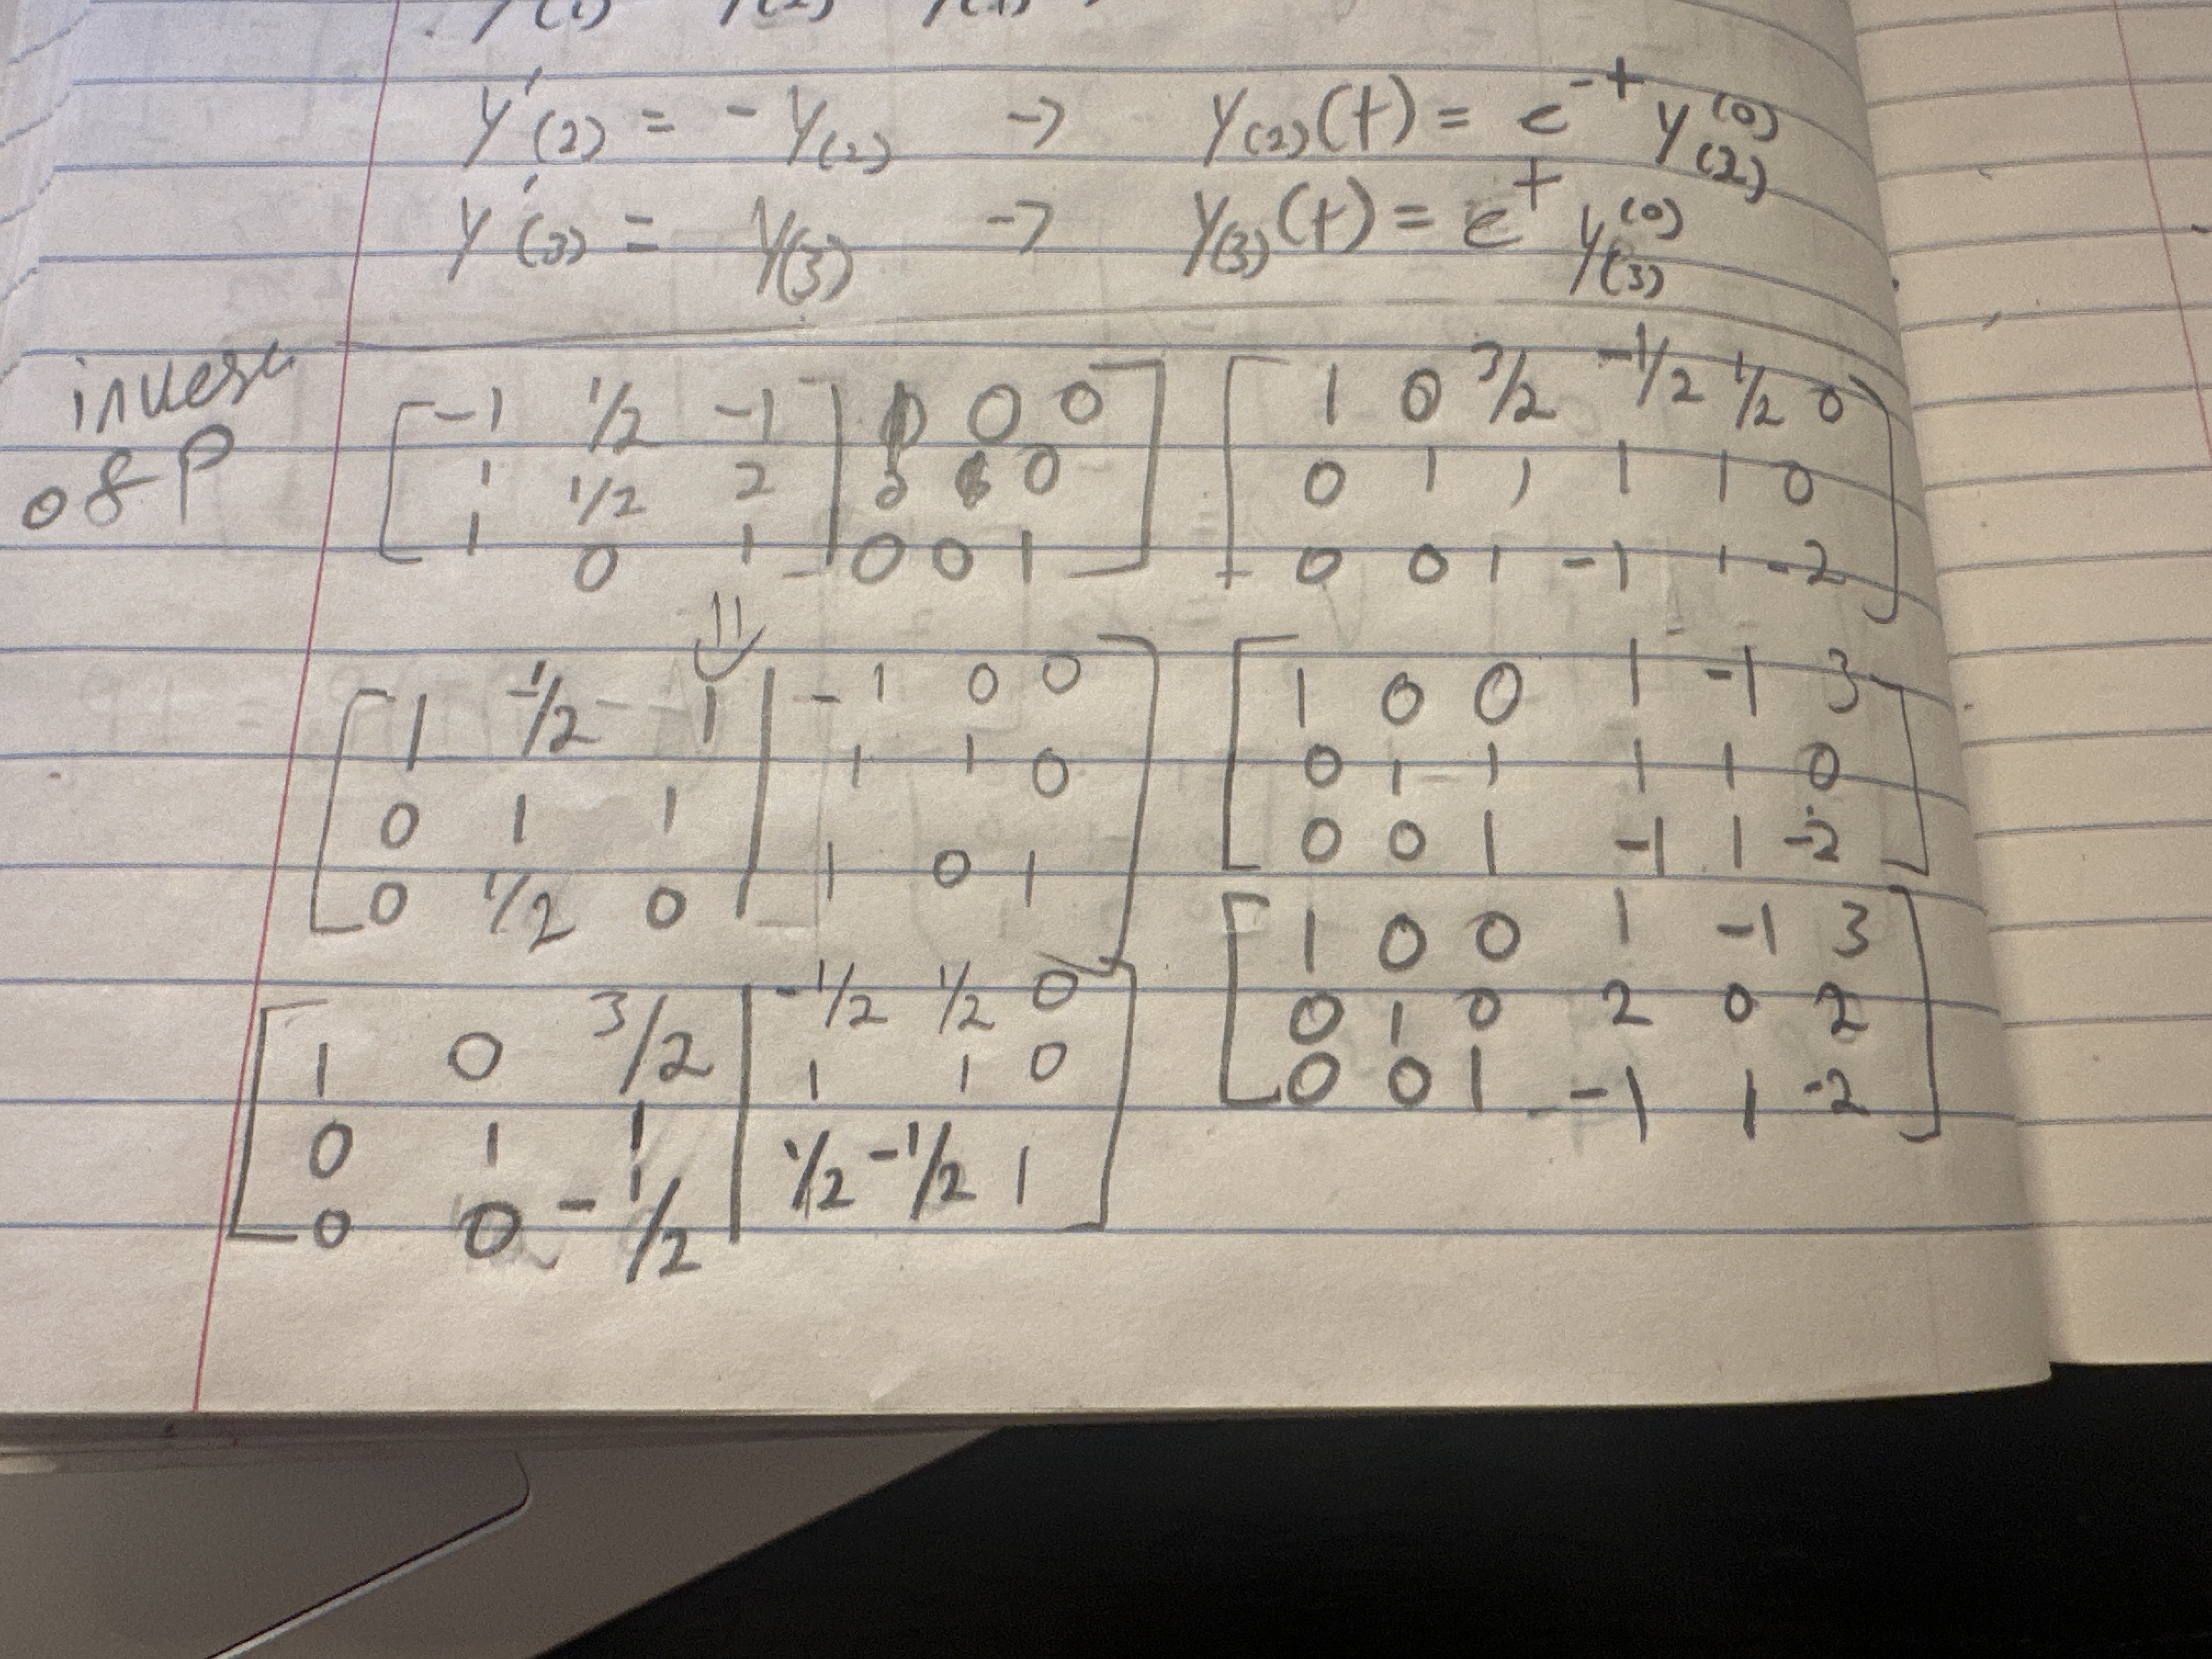
\includegraphics[width=\textwidth]{InverseP.JPG}
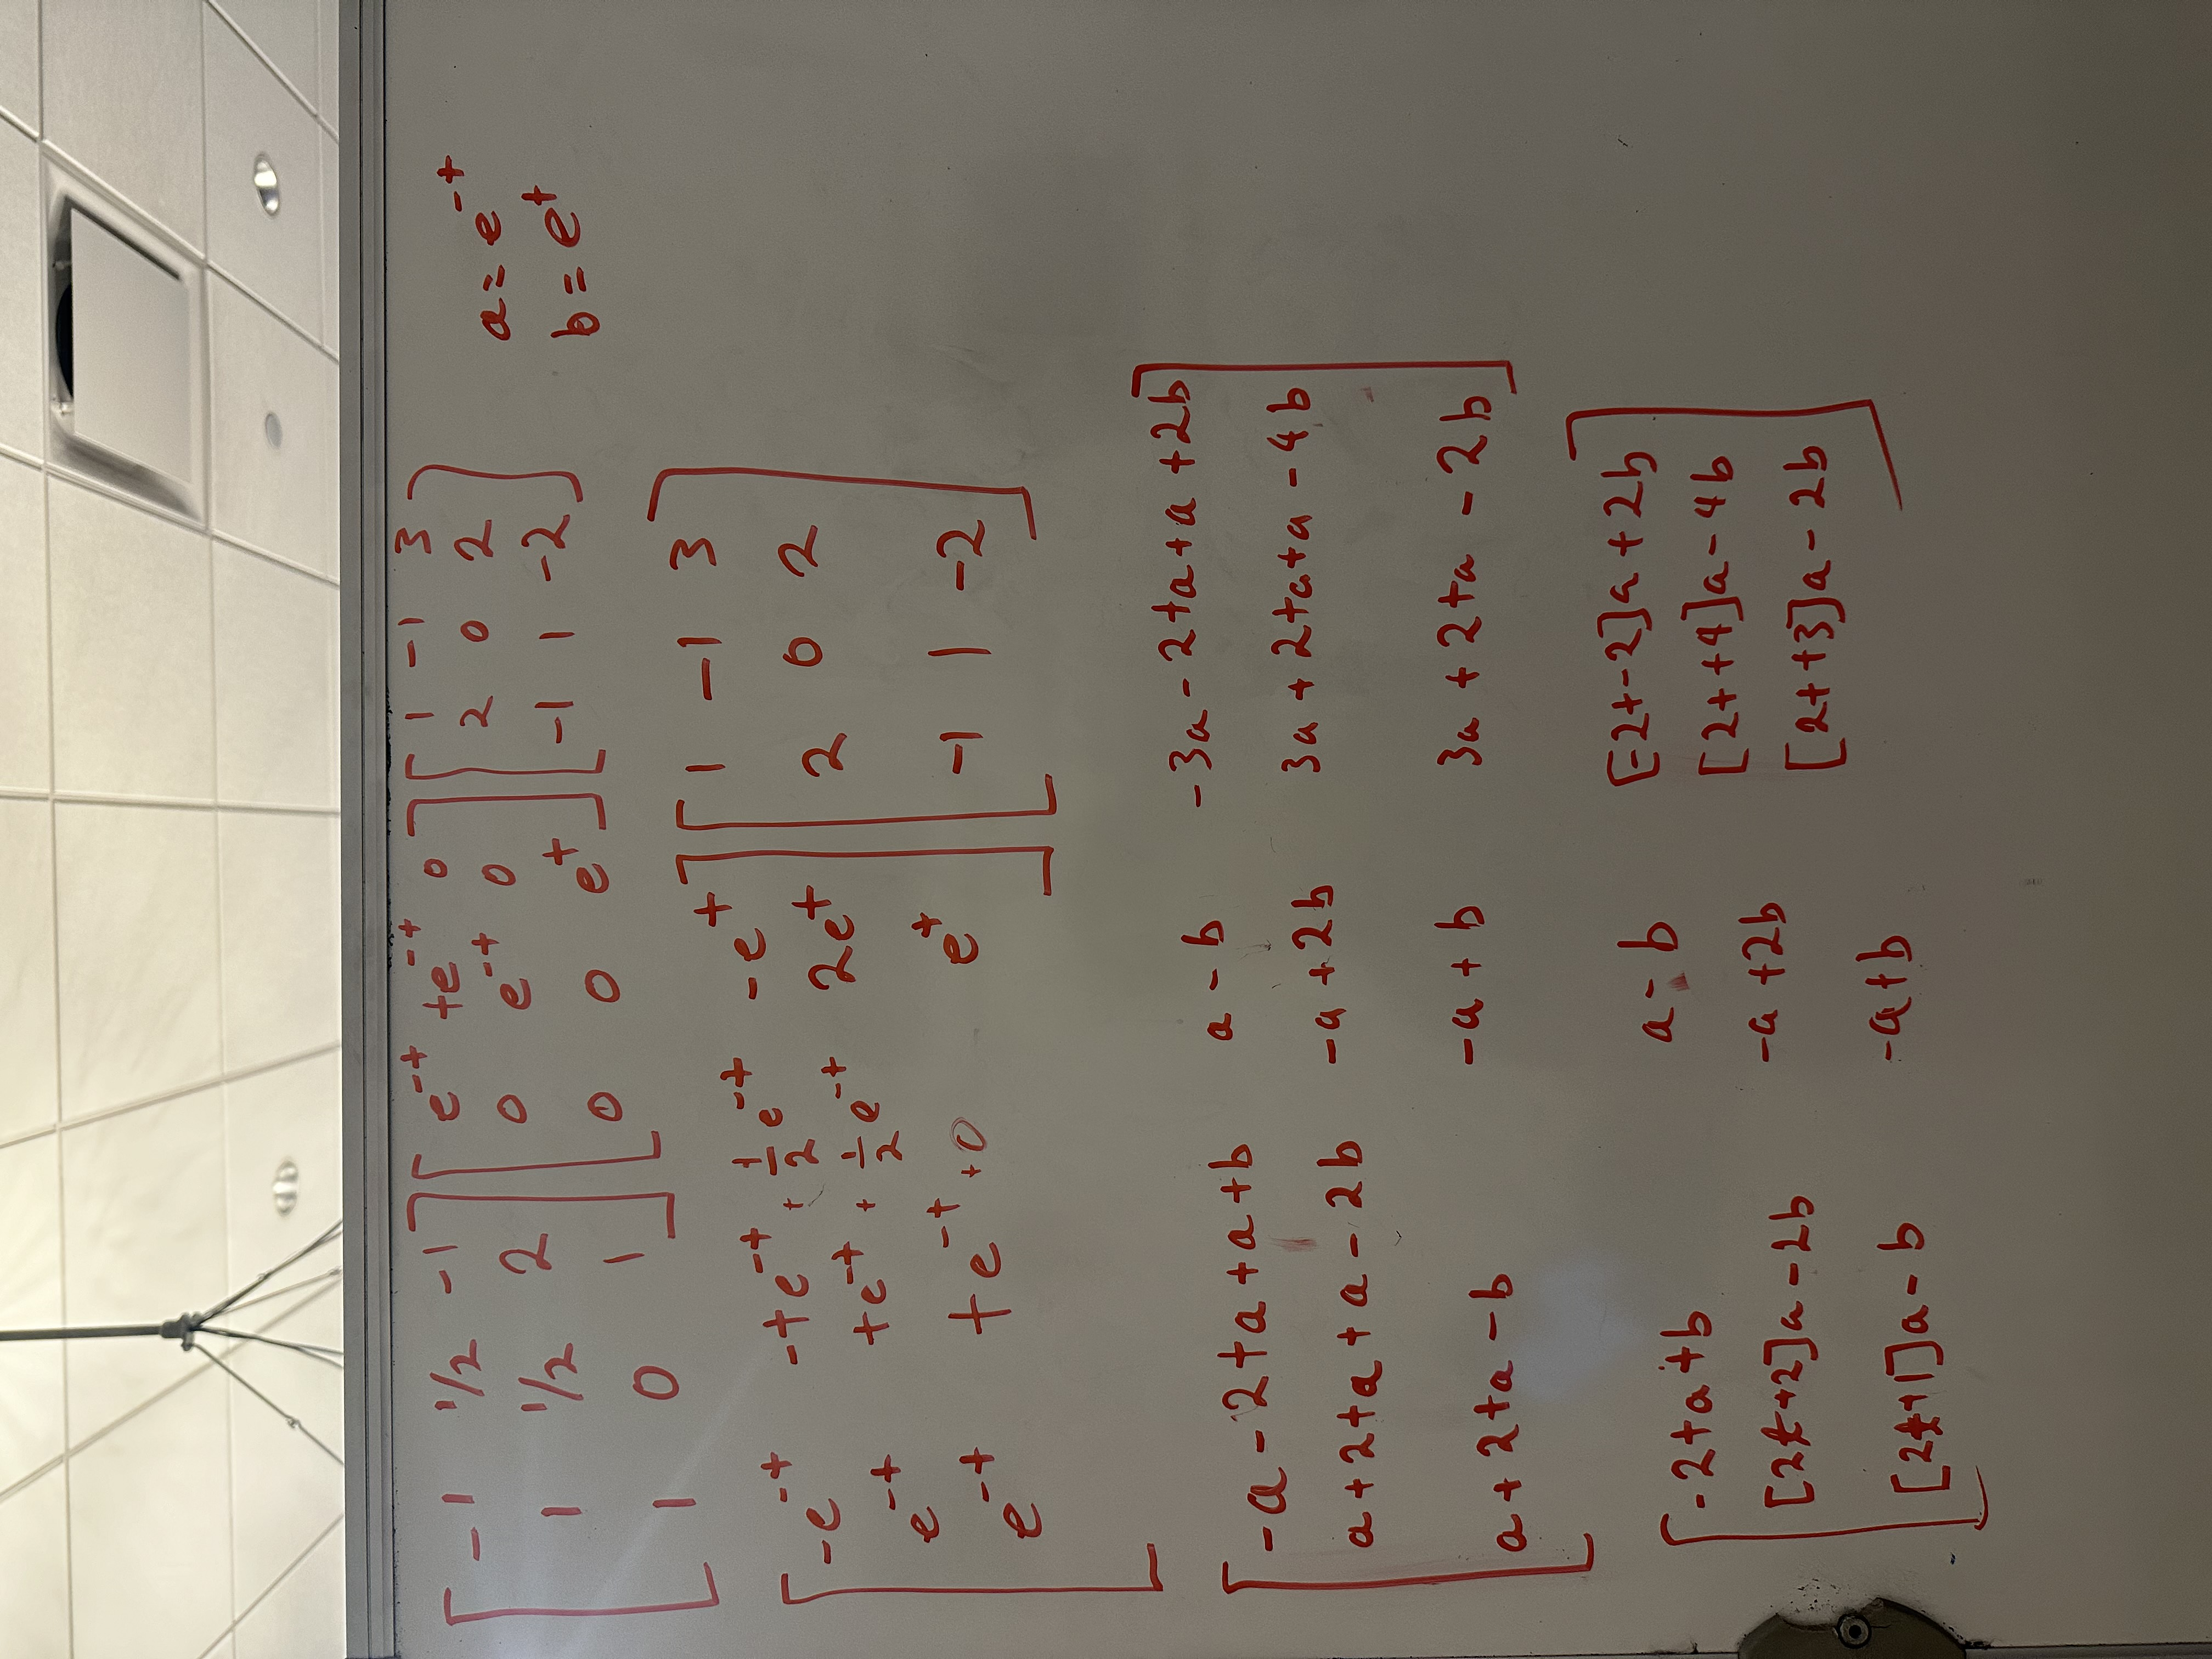
\includegraphics[width=\textwidth]{e^tA.JPG}

\end{document}